%%***********************************************
%% 		Setups
%%***********************************************
\documentclass[12pt, letterpaper, titlepage]{article}
%	\setlength{\columnsep}{31pt}		% space b/w columns;

% margins
\usepackage[top=.5in, bottom=1.2in, left=.7in, right=.7in]{geometry}

% title
\title{\Huge CSE 105: \\ Computation
	   \\[-1em] \rule{.8\textwidth}{1pt}
}
\author{\LARGE{\it by} Liu Tan}
\date{}
%\thanks{}

%***********************************************
% 		Graphs
%***********************************************

%% space of caption and the context;
%	\setlength{\abovecaptionskip}{10pt}
%	\setlength{\belowcaptionskip}{15pt}
%\usepackage{subfigure}
\usepackage{graphicx}
	\graphicspath{{pics/}}

%% figures with text wrapped around;
%\usepackage{wrapfig}
%\usepackage{picins}

\usepackage{tikz}
%	\usetikzlibrary{arrows}
%%\usepackage{tkz-euclide}
%\usepackage{pgfplots}
%	\tikzset{
%	myvec/.style={blue, line width = .5pt, -stealth'},
%	every node/.style={black},
%	box/.style={rectangle, rounded corners=5pt,
%			minimum width=30pt, minimum height=15pt,
%			inner sep=5pt,
%			draw=silver, fill=lightpurple},
%	}

% trees
\usepackage{tikz-qtree}
% \usepackage{pst-tree}

%% set wallpaper
%\usepackage{wallpaper}
%	\CenterWallPaper{1}{}

%% Include movies
%\usepackage{media9}

%% use colors
\usepackage{xcolor}
	\definecolor{lightblue}{RGB}{39, 104, 192}
	\definecolor{silver}{RGB}{200,191,231}
	\definecolor{lightpurple}{RGB}{200,200,240}

%%***********************************************
%% 		Tables
%%***********************************************

%% tables w/ wrapped lines;
%\usepackage{tabularx}
%	\newcommand{\ahsize}[1]{ \setlength{\hsize}{#1\hsize} }
%	\newcommand{\bhsize}[1]{ \setlength{\hsize}{#1} }

%% sideways
\usepackage{rotating}

%% makecell
%\usepackage{makecell}
%	\makegapedcells
%	\setcellgapes{6pt}

%% color for tables;
%\usepackage{colortbl}
%% toprule, midrule & bottomrule;
%\usepackage{booktabs}
\usepackage{array} %解决前置命令问题;
	\newcommand{\PreserveBackslash}[1]{\let\temp=\\#1\let\\=\temp}
	\newcolumntype{C}[1]{>{\PreserveBackslash\centering}p{#1}}
	\newcolumntype{R}[1]{>{\PreserveBackslash\raggedleft}p{#1}}
	\newcolumntype{L}[1]{>{\PreserveBackslash\raggedright}p{#1}}
	\newcolumntype{M}[1]{>{$}#1<{$}}

%% multirow;
\usepackage{multirow}

%% long table + tabularx;
%\usepackage{ltxtable, filecontents}

%%***********************************************
%% 		Coding
%%***********************************************

%	\usepackage{listings}
%		\lstset{
%			language=C++,
%			breaklines=true,				%自动换行;
%			extendedchars=false,			%这一条命令可以解决代码跨页时,章节标题,页眉等汉字不显示的问题;
%			numbers=left,
%			numberstyle=\scriptsize,
%			stepnumber=2, 				%行标跳过数;
%			numbersep=1.5em, 				%行标与代码框距离;
%			tabsize=4,
%			basicstyle=\footnotesize\ttfamily,
%			stringstyle=\color{lightblue},
%			keywordstyle=\color{blue!80},
%			commentstyle=\color{red!70!green!70!blue!90},
%			frame=shadowbox,
%%			showspaces=false,
%			showstringspaces=false,
%			showtabs=false,
%			rulesepcolor=\color{red!20!green!20!blue!20},
%			backgroundcolor=\color{red!10!green!3!blue!10},
%			escapeinside=``,
%			xleftmargin=8em,
%			xrightmargin=5em,
%			framexleftmargin=2pt,
%			framexrightmargin=2pt,
%			aboveskip=1em
%		}
%		\renewcommand{\lstlistingname}{CODE}

%***********************************************
% 		Fonts
%***********************************************

%% English;
\usepackage{fontspec}
	\setmainfont[Mapping=tex-text]{Times New Roman}
	\setsansfont[Mapping=tex-text]{Calibri}
	\setmonofont{Courier New}
%	\newfontfamily\rh{Lucida Handwriting}	% rh for Round Handing
%	\newfontfamily\sc{John Handy LET}	% sc for script
%	\newfontfamily\hw{Bradley Hand ITC}	% hw for HandWritting
%% Chinese;
%\usepackage[CJKchecksingle, CJKnumber]{xeCJK}
%	\setCJKmainfont[BoldFont = {STXingkai}, ItalicFont = {STFangsong}]{Microsoft YaHei}
%	\setCJKsansfont{}
%	\setCJKmonofont{KaiTi}
%	\punctstyle{hangmobanjiao}
%\newcommand{\CJKdash}{\rule[3.5pt]{9pt}{.77pt} \hspace{-1.5mm} \rule[3.5pt]{9pt}{.77pt} }

%%***********************************************
%% 		Looking
%%***********************************************

%% links
\usepackage[bookmarksnumbered, pdfencoding=auto, pdfborder=1, breaklinks,
			colorlinks, linkcolor=lightblue, urlcolor=blue]{hyperref}
	\hypersetup{
		unicode=false,			% non-Latin characters in Acrobat’s bookmarks
		pdftoolbar=true,		% show Acrobat toolbar?
		pdfmenubar=true,		% show Acrobat menu?
		pdftitle={},			% title
		pdfauthor={Jinyao Yuan},% author
		pdfsubject={},			% subject of the document
		pdfcreator={Jinyao Yuan},	% creator of the document
		pdfproducer={Jinyao Yuan},	% producter of the document
		citecolor=green,		% color of links to bibliography
		filecolor=magenta,		% color of file links
	}

%% page style
%%---------------------------------------------------------------------------
\usepackage{fancyhdr}
\pagestyle{fancy}
\lhead{}
\chead{}
\rhead{}
\renewcommand{\headrulewidth}{0pt}
\renewcommand{\footrulewidth}{0pt}
\lfoot{}
\cfoot{}
\rfoot{\thepage}

%% paragraphs
%%---------------------------------------------------------------------------
\usepackage{setspace}
	\onehalfspacing
%	\doublespacing
	\setlength{\parindent}{2em}
	\addtolength{\parskip}{3pt}
	\usepackage{indentfirst}

%% floats
%%---------------------------------------------------------------------------
% \renewcommand{\textfraction}{0.15}
% \renewcommand{\topfraction}{0.85}
% \renewcommand{\bottomfraction}{0.65}
\renewcommand{\floatpagefraction}{0.70}

\usepackage[section]{placeins}
% \usepackage[below]{placeins}
\usepackage{caption}

%% underline
%%---------------------------------------------------------------------------
% \usepackage{ulem}
%% \uline{加下划线}
%% \uwave{加波浪线}则是在文本下面加上波浪线。
%% \sout{中间加横线}

% \usepackage{CJKfntef}

%% emphasize style
%%---------------------------------------------------------------------------

\makeatletter
\DeclareRobustCommand{\em}{%
    \@nomath\em
    \if b\expandafter\@car\f@series\@nil \normalfont
    \else \bfseries \itshape
    \fi
}
\makeatother

% \DeclareTextFontCommand{\emph}{\em}

%% convert terms into Chinese;
%%---------------------------------------------------------------------------
%\renewcommand{\contentsname}{\hfill 目~录 \hfill}
%\renewcommand{\listfigurename}{图目录}
%\renewcommand{\listtablename}{表目录}
%\renewcommand{\thepart}{\CJKnumber{\arabic{part}}}
%\renewcommand{\partname}{第\CJKnumber{\thepart}章}
%\renewcommand{\thesection}{\CJKnumber{\arabic{section}}}
%\newcommand{\sectionname}{\thesection 节}
%\renewcommand{\figurename}{图}
%\renewcommand{\figureautorefname}{图}
%\renewcommand{\tablename}{表}
%\renewcommand{\tableautorefname}{表}
%\renewcommand {\thefootnote}{\arabic{footnote}}
%\renewcommand{\footnoteautorefname}{脚注}
%\renewcommand{\abstractname}{摘 \quad 要}
%\renewcommand{\appendixname}{附录{\thechapter}}
%\renewcommand{\appendixautorefname}{附录}
%\renewcommand{\bibname}{参考文献}
%\renewcommand{\indexname}{索引}

%% make own style of section titles;
%%---------------------------------------------------------------------------
\usepackage{titlesec}
%	\titleformat{\part}{\center\Huge \bf}{\thepart}{1em}{}
%	\titleformat{\section}{\large \bf}{\thesection}{1em}{}
	\titleformat{\part}[frame]{\normalfont}
		{\small \enspace UNIT \thepart \enspace}{6pt}
		{\LARGE\bf\filcenter}
	\titlespacing*{\part}{1pc}{*4}{*3}[1pc]
	\newcommand{\mypart}{\FloatBarrier\part}

%% make own style of table of contents;
%%---------------------------------------------------------------------------
%\usepackage{titletoc}
%\titlecontents{part}[0em]{\addvspace{10pt}\filright\bf\large}
%		{\def\numberline##1{\thecontentslabel\quad\ignorespaces}}
%		{}{\titlerule*[8pt]{.}\contentspage}
%\titlecontents{section}[1em]{\addvspace{10pt}\filright\bf\large}
%		{\def\numberline##1{\thecontentslabel\quad\ignorespaces}}
%		{}{\titlerule*[8pt]{.}\contentspage}
%\titlecontents{subsection}[2em]{\addvspace{5pt}\filright\bf}
%		{\def\numberline##1{\thecontentslabel\quad\ignorespaces}}
%		{}{\titlerule*[8pt]{.} \contentspage}

%***********************************************
% 		Utilities
%***********************************************

%% in-para enum, item, descript;
%%---------------------------------------------------------------------------
\usepackage{paralist}

%% lettrine;
%%---------------------------------------------------------------------------
%\usepackage{lettrine}
%	\newcommand{\mylettrine}[1]{\lettrine[lines=2,lraise=0,nindent=0em]{#1\hspace{1mm}}{}}

%% Math;
%%---------------------------------------------------------------------------
\usepackage{amsmath, amsfonts, amssymb, amsthm}
\usepackage{venndiagram}
%\usepackage{extarrows} 	% special arrows like \xlongequal;
%\input{longdiv.tex}	% divisions;
%\usepackage{dcolumn}	% vertical calculation w/ tabular;
\usepackage{cancel}	% strike out numbers

%% Theorems;
%%---------------------------------------------------------------------------
\newtheoremstyle{mystyle}
	{2em}	% spaceabove
	{2em}	% spacebelow
	{\it}	% bodyfont
	{0em}	% indent
	{\bf}	% headfont
	{}   	% headpunctuation
	{1em}	% headspace
	{%
		\thmname{#1} \thmnumber{#2} \thmnote{#3}.
	}   	% headspecify
\theoremstyle{mystyle}

\newtheorem{definition}{Definition}[section]
\newtheorem{theorem}{Theorem}[section]

%% symbols
%%---------------------------------------------------------------------------
\newcommand{\phteq}{ \phantom{{}={}} }
\renewcommand{\(}{ \left(  }
\renewcommand{\)}{ \right) }
\newcommand{\nth}{\ensuremath{^\text{th}} }
\newcommand{\st}{\ensuremath{^\text{st}} }
\newcommand{\nd}{\ensuremath{^\text{nd}} }
\newcommand{\rd}{\ensuremath{^\text{rd}} }
\newcommand{\dd}{{ \; \mathrm{d} }}
\newcommand{\abs}[1]{{ \left\lvert #1 \right\rvert }}

\newcommand{\set}[1]{{ \left\{\,#1\,\right\} }}
\newcommand{\lst}[1]{{ \left(\,#1\,\right) }}

%\newcommand{\dne}{ \mathrm{DNE} }	% Does Not Exist;
%\newcommand{\defeq}{ \xlongequal{\mathrm{DEF}} }	% equal by definition;
%\newcommand{\sqr}{ \ensuremath{^2} } % squared;
% \newcommand{\cels}{{ \ensuremath{^\circ \mathrm{C}} }}
%\newcommand{\fahr}{{ \ensuremath{^\circ \mathrm{F}} }}

\newcommand{\Conf}{{ \mathrm{Conf} }}
\newcommand{\true}{{ \text{\upshape True} }}
\newcommand{\false}{{ \text{\upshape False} }}

%%
\newcommand{\DFA}{{ M = \lst{Q, \Sigma, \delta, s, F} }}
\newcommand{\NFA}{{ N = \lst{Q, \Sigma, \delta, s, F} }}
\newcommand{\rev}{{ \mathrm{rev} }}
\newcommand{\combination}{{ \mathrm{C} }}
\newcommand{\permutation}{{ \mathrm{P} }}
\newcommand{\variance}[1]{{ \mathrm{Var}(#1) }}
\newcommand{\stirling}{ \mathrm{S} }
\newcommand{\powerset}{ \mathcal{P} }
\newcommand{\Degree}{ \mathbb{Deg} }
\newcommand{\degree}{ \mathbb{deg} }

%% visiblespace
\renewcommand\textvisiblespace[1][.5em]{%
	\makebox[#1]{%
		\kern.07em
		\vrule height.3ex
		\hrulefill
		\vrule height.3ex
		\kern.07em
	}
}

%% fillable forms
%%---------------------------------------------------------------------------
%\newcommand{\fform}[2]{
%#1 \vbox{\hbox{\TextField[name=#1,width=#2,borderwidth=0]{\null}}\kern0pt\hrule}
%}

%% Margin notes;
%%---------------------------------------------------------------------------
\usepackage{marginnote}
\marginparsep 2em
\marginparwidth 2.5in

% fancy boxes like \fbox,\shadowbox,\doublebox,\ovalbox, \Ovalbox。
\usepackage{fancybox}

%%***********************************************
%%	Self-defined environments
%%***********************************************

\usepackage{float} % used to define float environments

%% list point
%%---------------------------------------------------------------------------
%\newcommand{\lspnt}[1]{&\textrm{#1}}
%\newenvironment{pntlist} {
%	$
%	\left\{
%	\begin{aligned}
%}{
%	\end{aligned}
%	\right.
%	$
%}

%% centered graph
%%---------------------------------------------------------------------------
\newcommand{\centgraph}[2][.7\linewidth]{
	\begin{center}
		\includegraphics[width=#1]{#2}
	\end{center}
}

% \myfigure{Example of NFA}{pics/mp/nfa-0.pdf}
% \myfigure[width=1cm]{Example of NFA}{pics/mp/nfa-0.pdf}
\newcommand{\myfigure}[3][]{
    \begin{figure}[htbp]
        \centering
        \includegraphics[#1]{#3}
        \caption{#2}
    \end{figure}
}

%% simplified figure with label
% \myFigure[width=1cm]{Example of NFA}{exa:a}{pics/mp/nfa-0.pdf}
% \myFigure{Example of NFA}{exa:ab}{pics/mp/nfa-0.pdf}
\newcommand{\myFigure}[4][]{
    \begin{figure}[htbp]
        \centering
        \includegraphics[#1]{#4}
        \caption{#2}
        \label{#3}
    \end{figure}
}


%% questions & solutions
%%---------------------------------------------------------------------------
%\input{environment.question/quest.tex}

% shadowpage
%---------------------------------------------------------------------------
\newenvironment{shadowpage}%
{
	\begin{Sbox} \begin{minipage}
	}{
	\end{minipage} \end{Sbox}
	\setlength{\fboxsep}{10pt}
	\shadowbox{\TheSbox}
}%

% examples
%---------------------------------------------------------------------------

%\floatstyle{plaintop}
%\newfloat{exp}{htb}{log}[subsection]
%\floatname{exp}{Example}
\DeclareCaptionType[%
	placement=htbp,
	within=section,
	fileext=loe
]{myExample}[Example][List of Examples]
\newenvironment{example}[1][~]%
{%
	\begin{myExample}
		\hfill
		\begin{Sbox}
			\begin{minipage}{.8\linewidth}
				\footnotesize
				\vspace{-.5em} \caption{#1} ~ \\[-2em]
				\rule{\linewidth}{.3pt}
				\par
				\setlength{\parindent}{2em}
				\addtolength{\parskip}{3pt}
			}{%
			\end{minipage}
		\end{Sbox}
		\setlength{\fboxsep}{10pt}
		\shadowbox{\TheSbox}
	\end{myExample}
}%

%\newenviornment{keyword}

%\newenvironment{example}%
%{
%	\par\noindent
%	\hfill
%	\begin{Sbox}
%	\begin{minipage}{.8\linewidth}
%	\footnotesize
%	{\bf Example} \\[-1em]
%	\rule{\linewidth}{.5pt}
%	\par
%	\setlength{\parindent}{2em}
%}{
%	\end{minipage}
%	\end{Sbox}
%	\setlength{\fboxsep}{10pt}
%	\fbox{\TheSbox}
%	\par
%}%




%***********************************************
% 		START
%***********************************************
\begin{document}

\maketitle
%% 页码:目录使用罗马数字,正文阿拉伯
\renewcommand{\thepage}{\roman{page}}\setcounter{page}{1}
\tableofcontents\clearpage
\renewcommand{\thepage}{\arabic{page}}\setcounter{page}{1}


\section{Deterministic Finite Automaton (DFA)}
% ======================================================

A machine consists different drawn in circles with names. Often a state drawn as
a double circle is an ``acceptive state,'' and a plain circle indicates a
rejective state. A machine receives a string consisted of `1's and `0's as input
and the states change as the machine read through input digits. An arrow is used
to indicate which state is to start with. See \autoref{exa:a_DFA} for detailed
information.

\begin{example}[A DFA]
    \label{exa:a_DFA}

    Let's first look at the DFA below which starts at state $A$.
    \centgraph{pics/mp/dfa-0.pdf}

    If the string ``010110'' is input to the machine, will it result in true or false?
    Will the State be acceptive or rejective?
    \[
        \xrightarrow{010110}
        \fbox{M}
        \xrightarrow{ 1/0 \text{(True/False, Accept / Reject)} }
    \]

    There are two arrows leaving state $A$: one with a label reading `1' which points to
    state $B$ and one reading `0' which goes back to state $A$ itself. That means, if an
    input digit reads `1,' the state changes to B, and if `0' the state stays in $A$

    Now step through the procedure:
    \begin{compactenum}
    \item
        The machine starts off at state A with input `0,' which, as explained above,
        changes the state to $A$ itself.
    \item
        Next, the second digit `1' is read so the state is changed to $B$.
    \item
        The next difit `0' makse the state B to switch to state $C$
    \item
        Then state $C$ reads `1' so no state change occurs.
    \item
        The next digit is `1' again so the state remains still on $C$.
    \item
        Last, the digit `0' switches the state from $C$ to $B$.
    \end{compactenum}
    Thus the input string ``010110'' changes the machine to state $B$, which is an
    acceptive state.

\end{example}

\begin{definition}[DFA]
    \label{def:DFA}

    A DFA is a 5-turple
    \[
        M = (Q, \Sigma,\delta,s,F)
    \]
    where
    \begin{compactdesc}
    \item[$Q$]      is a finite set,     for states
    \item[$\sigma$] is a finite set,    for input alphabet
    \item[$s$]      $\in Q$,            for start states 
    \item[$F$]      $\subseteq Q$,      for accepting states
    \item[$\delta$]
        $Q \times \Sigma \mapsto Q$,
        a function that specifies the transition between states
    \end{compactdesc}
\end{definition}

\begin{example}[DFA table]
    \label{exa:DFA_table}
    According to definition \autoref{def:DFA},
    the machine in \autoref{exa:a_DFA} can be denoted by
    \[
        M = (Q, \Sigma,\delta,s,F)
    \]
    where
    \begin{compactitem}
    \item $Q = \{ A,B,C \}$
    \item $\Sigma = \{ 0,1 \}$
    \item $s = \{ A \}$
    \item $F = \{ B,C \}$
    \end{compactitem}
    And function $\delta$ can be described by the table below.
    \begin{center}
        \begin{tabular}{Mc Mc Mc}
        \hline
        \delta  & 0 & 1 \\
        \hline
        A       & A & B \\
        B       & C & A \\
        C       & B & C \\
        \hline
        \end{tabular}
    \end{center}

\end{example}

\begin{definition}[$f_M$]
    For and DFA $ M = (Q,\Sigma,\delta,s,F) $,
    let
    \[
        f_M: \Sigma^* \mapsto \{ \text{True}, \text{False} \}
    \]
    where $\Sigma^*$ is a set of string over $\Sigma$.

    \[
        f_M(w)
        = \begin{cases}
            \text{True},  & \delta^*(s,w) \in F \\
            \text{False}, & else
        \end{cases}
    \]
\end{definition}

\begin{definition}[$\delta^*$]
    \[
        \delta^* : Q \times \Sigma^* \mapsto Q
    \]
    which is an inductive function defined as
    \[
        \begin{cases}
            \delta^*(q, \varepsilon) &= q \\
            \delta^*(q, aw)          &= \delta^*\( \delta(q,a), w\)
        \end{cases}
    \]
    where $(q \in Q, a \in \Sigma, w \in \Sigma^*)$
\end{definition}



\begin{definition}[Configuration]
    \[
        Conf = Q \times \Sigma^*
    \]
\end{definition}

\begin{definition}[Initial Configurations]
    The initial configuration of a machine $I_M(w) \in Conf$
    \[
        I_M(w) = (s,w)
    \]
\end{definition}

\begin{definition}
    The final configuration of a machine $H_M(w) \subseteq Conf$
    \[
        H_M = \{ (q,u) \mid q \in Q, u = \varepsilon \} 
    \]
\end{definition}

\begin{definition}
The output of a machine is a function that either ``True'' or ``False.''
    \[
        O_M: H_M \mapsto \{\text {True}, \text {False}\}
    \]
    defined as
    \[
        O_M(q,\epsilon)
        = \begin{cases}
            \text{True},  & if \quad q \in F \\
            \text{False}, & if \quad q \notin F
        \end{cases}
    \]
\end{definition}

% ----------
In summary $\colon$
\begin{itemize}
\item F $\subseteq$ Q
\item s $\in$ Q
\item $\epsilon: Q \times \Sigma \mapsto Q$
\end{itemize}
% ----------

\begin{example}[\autoref{exa:a_DFA} as configurations] 
    With input ``10010'' write in mathematical language, the confiuration of machine in
    \autoref{exa:a_DFA}:
    \begin{align*}
        I_M(10010) 
        = (A,10010)
        \rightarrow      (B,0010)
        \rightarrow      (C,010)
        \rightarrow      (B,10)
        \rightarrow      (A,0)
        \rightarrow      (A, \varepsilon) \in H_M
    \end{align*}
    And thus the out put 
    \[
        O_F(A,\varepsilon) = \text{False}
    \].

    The machine in fact will only accept integers that are \emph{not} multiples of 3.
\end{example}


\begin{definition}[]
    
    \[
        R_M \subseteq Conf \rightarrow_M 
        = \{ 
            (q,aw), \( \delta(q,a),w \) 
            \mid q \in Q, a \in \Sigma, w \in \Sigma^* 
        \}
    \]
\end{definition}


\begin{definition}[]
    \[
        f'_n(w) = O_F(C_n)
    \]
    e.g. 
    \[
        I_M(w) \rightarrow_M C_1 \rightarrow_M C_2 \rightarrow_M \dots \rightarrow_M 
        \in H_M
    \]
\end{definition}

% ------------------------------
for example
\begin{align*}
    L(M)   & = \{ w \in \Sigma^* \mid f_M(w) = \text{True}\} \\
    L(M_1) & \neq \Sigma^*   \\
      1001 & \notin 3\times \mathbb{Z}
\end{align*}







\subsection{Languages}
% ------------------------------------------------------------
A subset of $\Sigma^*$ of a DFA that contains all inputs to which the output of the
machine is \true is called the \emph{language} of the machine.


In other word, If $A$ is the set of all strings that machine $M$ accepts, we say that $A$
is the \emph{ language of machine $M$} and write $L(M) = A$. ($M$ \emph{recognizes} $A$)

\begin{definition}[Regularity of Language]
    $ L \subseteq \Sigma^* $
    is regular if
    \[
        \exists {\text{\upshape DFA} M} \mid L(M) = L
    \]
\end{definition}

Which means, a DFA could \emph{recognize} L. In short, given a regular language, there
always exist a DFA could be draw.

Notice that 
\begin{itemize}
    \item
        $\varepsilon$(small epsilon) = \emph{ empty string } 
    \item
        $\Sigma$(big Sigma)          = \emph{ alphabet set } 
    \item
        $\varepsilon^*               = \set{\varepsilon}$  
    \item
        $\Sigma^*$                   = $\set{\varepsilon,1,0,10,101,\cdots} = \set{0,1}^*$,
\end{itemize}

\begin{example}[Which of the follwing languages are regular?]
    Given that
    and
    which of the following languages are regular?
    \begin{compactitem}
%     \item
%         $L_1 = \set{ w \in \set{0,1}^* \mid w \text{ is not a multiple of } 3}$,
    \item
        $L_1 = \set{ w \in \set{0,1}^* \mid w \text{ is a power of } 2}$, and
    \item
        $L_2 = \set{ w \in \set{0,1}^* \mid w \text{ is a power of } 3}$.
    \end{compactitem}
    
    $L_1$ is regular while $L_2$ is not. A binary number that is a power of $2$ consists
    of only one $1$ and all other digits should be $0$s. A DFA that recognizes the
    language would be
    \centgraph{mp/dfa-1.pdf}

\end{example}

\begin{definition}[Operations on Languages] \ \\
    \begin{compactdesc}
    \item[Complement]
        $L^C = \set{w \in \Sigma^* \mid w \notin L}$
    \item[Union]
        $L_1 \cup L_2 = \set{w \in \Sigma^* \mid w \in L_1 \vee w \in L_2}$
    \item[Intersection]
        $L_1 \cap L_2 = \set{w \mid w \in L_1 \wedge \in L_2}$
    \item[Concatenation]
        $L_1 \cdot L_2 = \set{w_1 \cdot w_2 \mid w \in L_1, w_2 \in L_2}$
    \end{compactdesc}
\end{definition}

\begin{theorem}
    \label{thm:R_closed_under_union}
    $\mathbb R$ is closed under complement.
\end{theorem}

\begin{example}[If $L$ is regular, is $L^C$ also regular?]
    Yes.

    \begin{proof}[Proof of \autoref{thm:R^C}]
        Let $L \in \mathbb R,$
        prove $L^C \in \mathbb R:$

        By definition, 
        \[
            \exists \DFA \text{ s.t.\ } L(M) = L.
        \]

        Let $M' = \lst{Q,\Sigma,\delta,s,F^C},$

        then $L(M') = L(M)^C = L^C.$

        $L^C \in \mathbb R$ because $L^C = L(M').$
    \end{proof}
\end{example}

\begin{example}[$\forall L_1, L_2$ \\ 
    $
        L_1 \in \mathbb R \vee L_2 \in \mathbb R
        \implies L_1 \cup L_2 \in \mathbb R
    $]
    \label{exa:R_closed_under_union}
        Yes, $\mathbb R$ is closed under union.
\end{example}



\section{Nondeterministic Finite Automaton (NFA)}
% ==================================================

\begin{example}[How many states needed?]
    \[
        L = \set{w \in \set{0,1}^* \mid
            \text{ the $5^{th}$ (from the left) of $w$ is $0$ } }
    \]
    We will need 7 states

    \centgraph{mp/dfa-2.pdf}

    What if
    \[
    L = \set{w \in \set{0,1}^* \mid
        \text{ the $5^{th}$  from the \emph right) of $w$ is $0$} }
    \]

    \centgraph{mp/dfa-3.pdf}
    Notice this is a \textbf{DFA}
\end{example}

\begin{definition}[NFA]
    \label{def:NFA}
    An NFA is a $5$-tuple
    \[
        N = (Q,\Sigma, \delta,s,F)
    \]
    where
    \begin{compactitem}
    \item $Q$ and $\Sigma$ are finite sets
    \item $s \in Q$
    \item $F \subseteq Q$
    \item $\delta \colon
        Q \times \Sigma_\varepsilon
        \footnote{$\Sigma_\varepsilon = \Sigma \cup \set{\varepsilon}$}
        \mapsto \powerset(Q)$

        $\delta(A,\varepsilon) = \set{H}$
        $\delta(D,\varepsilon) = \emptyset$

    \end{compactitem}

\end{definition}

% \begin{definition}[Configurations of NFA]
%     \begin{align*}
%         \Conf  &= Q \times \Sigma^* \\
% 
%         I_M(w) &= (s,w)             \\
% 
%         H_M(w) &= Q \times \set\varepsilon \\
% 
%         O_M(q,\varepsilon)
%         &= \begin{cases}
%             \true,  & if \quad q \in F \\
%             \false, & \text{otherwise}
%             \end{cases}\\
% 
%         R = \set{(q,aw) \mapsto (q',w) \mid
%             \forall q \in Q, a \in \Sigma_\varepsilon, w \in \Sigma^*}
%     \end{align*}
% \end{definition}

In DFA, only one output; 
In NFA, many possible ways from the same input.

    $C_0, C_1, \dots , C_n$
    Computation is a sequence of Configurations, such that $C_0 = I(w)$
    $\forall i, (C_i, C_{i+1} \in \mathbb{R})$ \\
    $[C_i \mapsto C_{i+1}], C_n \in H $ \\
% ---------------------------------------------------------------------
    \newpage

    \fbox{ 
    Accepting if $O(C_n)$ = \true 
    Rejecting if $O(C_n)$ = \false 
}

\begin{definition}[Language of NFA]
    \[
        L(N) = \set{w \mid \exists \text{accepting computation on input $w$} }
    \]
\end{definition}

\begin{theorem}
    \label{thm:NFA_to_DFA}
    \[
        \forall \NFA,\,
        \exists \text{\upshape DFA} \quad M = \lst{ Q', \Sigma', \delta', s', F'} \text{s.t.}
        L(N) = L(M)
    \]
\end{theorem}

\begin{proof}[Proof of \autoref{thm:NFA_to_DFA}]
    \begin{align*}
        Q' &= \powerset(Q) \\
        F' &= \set{ A \subseteq Q \mid A \cap F \neq \varnothing} \\
        s' &= E(\set{s})  = \set{q \in Q \mid \exists s
                                                \xrightarrow\varepsilon q_1
                                                \xrightarrow\varepsilon q_2
                                                \xrightarrow\varepsilon q_3
                                                \cdots 
                                                \xrightarrow\varepsilon q_n
        } \\
        \delta'(A, a) &= E( \operatorname*\cup_{q \in A} \delta (q,a) )
    \end{align*}
\end{proof}


\subsection{Equivalence of NFAs and DFAs}
% ------------------------------------------------------------

A finite automaton(DFA $\Longleftrightarrow$ NFA)

\begin{enumerate}
    \item Defining Models of computation.
    \item testifying equivalence between models.
\end{enumerate}

\begin{definition}[Reverse] \ \\
    \begin{compactitem}
    \item
        reverse of a string
            \[
                \rev\big( \lst{Q_1, Q_2, \cdots, Q_n} \big) = \lst{Q_n,  Q_(n-1), \cdots,
                Q_1}.
            \]
    \item
        reverse of a language
            \[
                \rev(L) = \set{ rev(w) \mid w \in L }.
            \]
         \myfigure{Example of NFA}{pics/mp/nfa-2.pdf}
    \end{compactitem}
\end{definition}

It is easy to find out that 
\[
    \forall L \in \mathbb R, \rev(L) \in \mathbb R.
        \footnote{$\mathbb R $ = Regular language}
\]

\begin{example}[Regular language is closed under union]
    \label{exa:R_closed_under_union_with_NFA}

    Recall \autoref{exa:R_closed_under_union}, with NFA, we could proof
    \autoref{thm:R_closed_under_union} much more easier now.

    \begin{proof}[Proof of \autoref{thm:R_closed_under_union}]
        Let $M_1, M_2$ become NFA for $L_1$ and $L_2$.
        We build a NFA for $L_1 \cup L_2$
        by simply adding a new initial state that transit to $s_1$ and $s_2$ with
        $\varepsilon$ arrows:
        \centgraph[3cm]{pics/mp/nfa-3.pdf}
    \end{proof}
\end{example}



\begin{example}[Regular language is closed under concatenation]
    \begin{proof}
        Let $M_1, M_2$ become NFA for $L_1$ and $L_2$.
        We build a NFA for $L_1 \circ L_2$:
        \begin{compactenum}
        \item Assign M's start to be the start state of $M_1$ which is $s_1$ and
        \item change the final states in $M_1$ to regular states and connect them to $s_2$
            with additional $\varepsilon$ arrows that nondeterministically allow branching
            to $M_2$ whenevr $M_1$ is in an accept state, signifying that it has found an
            initial piece of the input that constitues a string in $L_1$
        \item The accept states of $M$ are the accept states of $M_2$ only. only.
        \end{compactenum}
        See the graph for visualization:
        \begin{center}
            \begin{minipage}{4cm}
                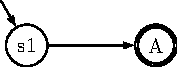
\includegraphics[width=\textwidth]{pics/mp/nfa-4.pdf}
                \center $M_1$
                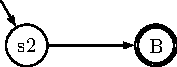
\includegraphics[width=\textwidth]{pics/mp/nfa-5.pdf}
                \center $M_2$
            \end{minipage}
            \; $\longrightarrow$ \;
            \begin{minipage}{4cm}
                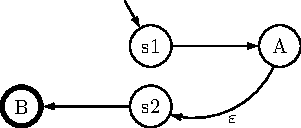
\includegraphics[width=\textwidth]{pics/mp/nfa-6.pdf}
                \center $M$
            \end{minipage}
        \end{center}
        thus 
        \[
            L(M) = L(M_1) \circ L(M_2)  = \set{wv \mid w \in L(M_1), v \in L(M_2)}
        \]
    \end{proof}
\end{example}




\end{document}

